% IEEE journal version (10 to 12 pages), two-column.
% Uses IEEEtran.cls V1.8b in journal mode, the class distributed with the
% official IEEE templates (https://www.ieee.org/conferences/publishing/templates;
% CTAN package ieeetran). Do not change margins, fonts, or column settings.
%
% Status: study design. No solver, PINN, or energy run exists yet.
% Sources of truth: docs/research-plan.md, docs/problem-definition.md,
% docs/model-equations.md, docs/reference-solution.md,
% docs/training-pipeline.md, docs/gap-analysis.md, docs/gap-evidence.md.
\documentclass[journal]{IEEEtran}

\usepackage{cite}
\usepackage{amsmath,amssymb,amsfonts}
\usepackage{graphicx}
\usepackage{textcomp}
\usepackage{xcolor}
\usepackage{booktabs}
\usepackage{array}
\usepackage{tikz}
\usetikzlibrary{positioning,arrows.meta,fit,calc}
\usepackage[hidelinks]{hyperref}
\graphicspath{{../shared/figures/}}

\newcommand{\Nstar}{N^{\ast}}

\begin{document}
\bstctlcite{IEEEexample:BSTcontrol}

\title{Reaching the Energy and Computational Break-Even Point Between PINNs, and Classical Solvers}

\author{Anonymous~Author(s)%
\thanks{Affiliation withheld for review.}}

\markboth{Study design, not yet peer reviewed}%
{Reaching the Energy and Computational Break-Even Point}

\maketitle

\begin{abstract}
A parametric physics-informed neural network (PINN) is trained once for a whole family of problems. After training, each new parameter setting needs only one forward pass. A classical solver must solve a new system for every setting. The PINN, however, spends energy on training before it gives its first answer. This paper asks how many new queries it takes before the PINN's total electricity falls to that of a finite-difference solver at the same accuracy. It asks the same question for runtime. Published comparisons of PINNs with classical solvers report time for single solves. Break-even studies cover supervised neural operators and count solves or seconds. In our search, none measures electricity across a parameter family. We present a study design for that measurement and list its open decisions. It reports no measured results. The workload is steady diffusion on the unit square, where two parameters set a varying conductivity. Both methods answer the same unseen parameters on one output grid, at relative L2 errors of 1\% and 0.1\%. The design has four parts. A cost model charges failed training runs and the cost of checking accuracy. An accuracy gate keeps any method that misses a target out of the cost comparison. A counter-based protocol reads both methods inside one energy boundary on one machine. A decision rule sorts each result into one of four outcomes, each with an uncertainty interval. A crossover that is absent, uncertain, or very far away is a valid result.
\end{abstract}

\begin{IEEEkeywords}
Physics-informed neural networks, energy measurement, green computing, finite differences, break-even analysis, parametric partial differential equations.
\end{IEEEkeywords}

% ===========================================================================
\section{Introduction}\label{sec:intro}

\IEEEPARstart{A}{physics-informed} neural network (PINN) learns the solution of a partial differential equation (PDE). It does this by making the equation's residual small at sampled points~\cite{raissi2019}. PINNs are now a large research area~\cite{karniadakis2021,cuomo2022,toscano2025}. This paper asks a cost question about them. When does the energy spent on training a PINN pay for itself?

\subsection{Why Training Cost Matters}
A parametric PINN takes the PDE parameters as extra inputs. One trained network then covers a whole family of problems~\cite{sun2020,wang2021deeponet}. To answer a new parameter setting, the network runs one forward pass. A classical solver has no training step. It must, however, solve a new linear system for every setting. So the two methods spend their effort at different times. The PINN pays a large cost up front and a small cost per query. The classical solver pays a small cost up front and a larger cost per query.

This pattern suggests a crossover. After enough queries, the PINN's total cost might fall below the solver's total cost. Whether this happens is not obvious. It depends on how large the training cost is, how cheap each PINN query is, and how cheap each classical solve is. It also depends on the accuracy required. Work on green computing asks that such energy costs be measured and reported, not assumed~\cite{strubell2019,schwartz2020,patterson2022}. The energy of answering queries also adds up over time~\cite{luccioni2024}.

\subsection{What Published Work Tells Us}
In the search recorded for this project, we found no published study that settles the question. Studies that compare PINNs with classical solvers time one problem at a time~\cite{grossmann2024,chuang2022,markidis2021}. Grossmann et~al. found the finite element method faster than PINNs at equal or better accuracy in nearly every test~\cite{grossmann2024}. Their paper also names parameterized PDEs as a case it did not study. In two of these studies, the training time of the PINN was reported next to the time of one classical solve. Dividing one by the other gives ratios from about 69~\cite{markidis2021} to more than 28\,000~\cite{chuang2022}. These ratios come from PINNs trained for one problem. Our PINN is trained once for a whole family, so the ratios do not predict our result. They do show how far apart the published numbers are.

Studies of many queries focus on supervised neural operators. One preprint reports that no Fourier neural operator with error below 1\% broke even before about 31\,000 queries~\cite{huang2026review}. Another preprint defines break-even for neural solvers in wall-clock time~\cite{zhang2026}. Neither study uses a PINN. Neither measures energy. The closest energy studies estimate carbon with software tools~\cite{kapoor2025} or meter the inference of a neural operator alone~\cite{yoo2026}.

Simple proxies for energy can mislead. Across model architectures, floating-point operation counts explained little of the variation in energy ($R^2=0.083$)~\cite{henderson2020}. In a PDE forecasting preprint, runtime alone was an unreliable proxy for carbon cost, especially during training~\cite{wilson2025}. A faster method may still use more energy. So we measure the energy crossover and the runtime crossover separately.

\subsection{What Makes a Fair Measurement Hard}
Three problems stand in the way of a fair answer.

The first problem is the baseline. A crossover only means something if both methods reach the same accuracy and the classical solver is efficient. McGreivy and Hakim reviewed papers that claimed to beat a standard numerical method. In 79\% of them, the baseline was weak~\cite{mcgreivy2024}.

The second problem is the measurement boundary. The two methods may run on different devices. Grossmann et~al. ran the PINN on a GPU and the classical solver on CPU cores of the same machine~\cite{grossmann2024}. Chuang and Barba used different machines~\cite{chuang2022}. A GPU reading and a CPU reading are not the same system total. Energy must be read inside one declared boundary for both methods.

The third problem is training failure. PINN training can stall or fail~\cite{krishnapriyan2021,wang2022ntk,rathore2024}. A failed run still uses energy. If only the best run is counted, the training cost looks smaller than it is.

\subsection{What This Paper Does}
This paper sets out a study design that handles these three problems for one workload. The workload is 2D steady diffusion with two conductivity parameters, solved on one machine. The paper reports no measured results. Its contributions are:
\begin{itemize}
\item a break-even cost model for energy and runtime that charges failed training runs and the cost of checking accuracy, with a rule that sorts each result into one of four outcomes (Section~\ref{sec:model});
\item a design for a matched-accuracy comparison, with an accuracy gate on unseen parameters, a finite-difference solver that keeps all valid reuse, and a parametric PINN with exact boundary values and a logged training process (Sections~\ref{sec:setup}, \ref{sec:classical}, and~\ref{sec:pinn});
\item a measurement protocol that reads both methods inside one energy boundary, keeps setup, training, and query costs apart, and logs every run in a study ledger (Section~\ref{sec:measure}).
\end{itemize}

Fig.~\ref{fig:pipeline} shows the whole study. Section~\ref{sec:related} reviews related work. Section~\ref{sec:setup} defines the problem and the accuracy gate. Section~\ref{sec:model} builds the cost model. Sections~\ref{sec:classical} and~\ref{sec:pinn} describe the two solvers. Section~\ref{sec:measure} gives the measurement protocol. Section~\ref{sec:pilot} lists the pilot checks, and Section~\ref{sec:report} shows how results will be reported. Section~\ref{sec:threats} discusses threats to validity, and Section~\ref{sec:open} lists open decisions. Section~\ref{sec:conclusion} concludes.

\begin{figure*}[t]
\centering
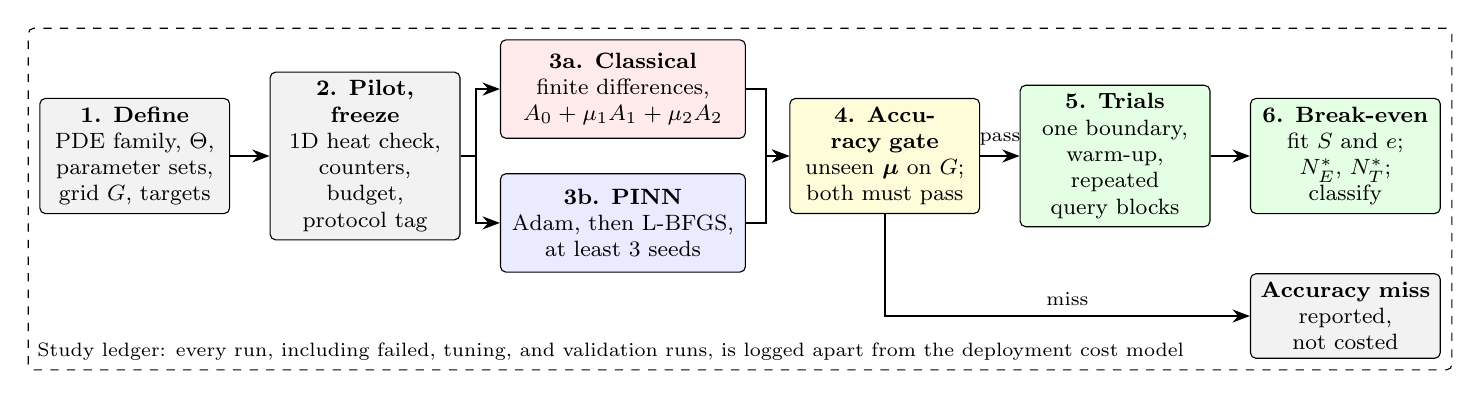
\begin{tikzpicture}[
  font=\footnotesize,
  >={Stealth[length=2.2mm]},
  box/.style={draw, rounded corners=2pt, align=center, text width=2.2cm, minimum height=1.25cm, inner sep=3pt, fill=#1},
  box/.default=white,
  arr/.style={->, thick},
  node distance=0.5cm
]
\node[box=gray!10] (def) at (0,0) {\textbf{1. Define}\\ PDE family, $\Theta$,\\ parameter sets,\\ grid $G$, targets};
\node[box=gray!10, right=of def] (pilot) {\textbf{2. Pilot, freeze}\\ 1D heat check,\\ counters, budget,\\ protocol tag};
\node[box=red!8, right=of pilot, yshift=0.85cm, text width=2.9cm] (fd) {\textbf{3a. Classical}\\ finite differences,\\ $A_0+\mu_1A_1+\mu_2A_2$};
\node[box=blue!8, right=of pilot, yshift=-0.85cm, text width=2.9cm] (pinn) {\textbf{3b. PINN}\\ Adam, then L-BFGS,\\ at least 3 seeds};
\node[box=yellow!15, anchor=west] (gate) at ($(fd.east)!0.5!(pinn.east)+(0.55,0)$) {\textbf{4. Accuracy gate}\\ unseen $\boldsymbol{\mu}$ on $G$;\\ both must pass};
\node[box=green!10, right=of gate] (trial) {\textbf{5. Trials}\\ one boundary,\\ warm-up, repeated\\ query blocks};
\node[box=green!10, right=of trial] (be) {\textbf{6. Break-even}\\ fit $S$ and $e$;\\ $\Nstar_E$, $\Nstar_T$;\\ classify};
\node[box=gray!10, below=0.75cm of be, minimum height=0.8cm] (fail) {\textbf{Accuracy miss}\\ reported, not costed};
\draw[arr] (def) -- (pilot);
\draw[arr] (pilot.east) -- ++(0.2,0) |- (fd.west);
\draw[arr] (pilot.east) -- ++(0.2,0) |- (pinn.west);
\draw[arr] (fd.east) -- ++(0.25,0) |- (gate.west);
\draw[arr] (pinn.east) -- ++(0.25,0) |- (gate.west);
\draw[arr] (gate) -- node[above, font=\scriptsize]{pass} (trial);
\draw[arr] (trial) -- (be);
\draw[arr] (gate.south) |- node[pos=0.75, above, font=\scriptsize]{miss} (fail.west);
\node[draw, dashed, rounded corners=2pt, fit=(def)(fd)(pinn)(be)(fail), inner sep=4pt, label={[font=\scriptsize, anchor=south west]south west:Study ledger: every run, including failed, tuning, and validation runs, is logged apart from the deployment cost model}] {};
\end{tikzpicture}
\caption{Study pipeline. The pilot ends in a frozen protocol. The two solvers are then built in parallel and meet at one accuracy gate on unseen parameters. Only targets that both methods pass go on to the energy and runtime trials. A miss is reported as a result.}
\label{fig:pipeline}
\end{figure*}

% ===========================================================================
\section{Background and Related Work}\label{sec:related}

This section follows the question from method to evidence. It starts with what a parametric PINN is. It then reviews what has been measured, what training costs, and how energy is measured. It ends with the gap that the study targets.

\subsection{PINNs and Parametric PINNs}
Raissi et~al. set out the PINN method~\cite{raissi2019}. A network is trained so that it fits the boundary data and makes the PDE residual small. Reviews cover the method's uses and its open problems~\cite{karniadakis2021,cuomo2022,toscano2025}. A parametric PINN adds the PDE parameters to the network inputs. Sun et~al. trained such a network for fluid flows without any simulation data. They also built the boundary conditions into the network~\cite{sun2020}. Wang, Wang, and Perdikaris trained physics-informed DeepONets for parametric PDEs, again without paired data~\cite{wang2021deeponet}. So a parametric PINN is not new. What is missing is a measured account of its total cost.

\subsection{PINNs Against Classical Solvers}
Table~\ref{tab:related} lists the closest studies. The project's evidence matrix gives the source of each cell. Grossmann et~al. compared PINNs with the finite element method on Poisson, Allen-Cahn, and Schr\"odinger problems~\cite{grossmann2024}. The finite element method was faster at equal or better accuracy in nearly every test. In one case, evaluating a trained PINN on a 3D Poisson problem was faster than finite element interpolation. Chuang and Barba compared a PINN with a finite-difference code on 2D flow problems~\cite{chuang2022}. Markidis compared PINNs with a conjugate gradient (CG) solver on Poisson problems~\cite{markidis2021}. All three studies measure time, and all three solve one problem at a time.

The physics-informed DeepONet was up to three orders of magnitude faster than a conventional solver per query~\cite{wang2021deeponet}. That speedup is for inference with a trained model. It does not include training.

\begin{table}[t]
\caption{Closest studies and what they measure}
\label{tab:related}
\centering
\footnotesize
\setlength{\tabcolsep}{2.5pt}
\begin{tabular}{@{}lllll@{}}
\toprule
Study & Model & Classical rival & Many queries & Cost \\
\midrule
Grossmann~\cite{grossmann2024} & PINN & FEM & No & Time \\
Chuang~\cite{chuang2022} & PINN & Finite diff. & No & Time \\
Markidis~\cite{markidis2021} & PINN & PETSc CG & No & Time \\
Wang~\cite{wang2021deeponet} & PI-DeepONet & Spectral & Yes & Query time \\
Huang~\cite{huang2026review}$^{\mathrm{a}}$ & FNO & FV, AMG-CG & Yes & Solves, time \\
Zhang~\cite{zhang2026}$^{\mathrm{a}}$ & Operators & Coarse num. & Yes & Time \\
Kapoor~\cite{kapoor2025}$^{\mathrm{a}}$ & PINN, ops. & None & Yes & Est. carbon \\
This design & PINN & Finite diff. & Yes & Time, joules \\
\bottomrule
\multicolumn{5}{@{}l}{$^{\mathrm{a}}$Preprint. Rows follow the project's evidence matrix.}
\end{tabular}
\end{table}

\subsection{What Published Times Say About the Crossover}
Our cost model appears in Section~\ref{sec:model}. Here we only need one simple case. Suppose a PINN query costs almost nothing and the classical setup is small. The crossover is then close to the ratio of PINN training time to one classical solve. Two of the single-solve papers report both numbers. Table~\ref{tab:ratios} shows the ratios we computed from them.

\begin{table}[t]
\caption{Ratios computed from published times (not our data)}
\label{tab:ratios}
\centering
\footnotesize
\setlength{\tabcolsep}{2.5pt}
\begin{tabular}{@{}llll@{}}
\toprule
Source & PINN training & Classical solve & Ratio \\
\midrule
Markidis~\cite{markidis2021} & 6380 s & 92.28 s (CG) & about 69 \\
Chuang~\cite{chuang2022}, abstract & about 32 h & under 20 s & over 5700 \\
Chuang~\cite{chuang2022}, $10^{-3}$ case & over 8 h & under 1 s & over 28\,000 \\
\bottomrule
\end{tabular}
\end{table}

These ratios need care. In Markidis, both methods ran on the same CPU, but CG ran to machine precision. A CG run stopped at the PINN's accuracy would take no longer, so the matched ratio would be at least 69. In Chuang and Barba, the two methods ran on different hardware. In both papers, the PINN was trained for one problem. A PINN trained for a whole family may cost more or less to train. No row in our evidence reports which. The ratios also measure time, not energy. They show that published numbers span more than two orders of magnitude, and that none of them is in joules.

\subsection{Many-Query Cost Studies}
De Hoop et~al. studied the trade-off between cost and accuracy in operator learning~\cite{dehoop2022}. Huang and Stuart, in a preprint, found classical solvers ahead of neural operators as the accuracy target tightens~\cite{huangstuart2026}. Huang et~al., also a preprint, give an amortization law for learned surrogates~\cite{huang2026review}. In their tests, the classical baseline was a finite-volume solver with algebraic multigrid preconditioned CG, and the models were trained with three seeds. Zhang et~al. define break-even complexity for neural PDE solvers in wall-clock time~\cite{zhang2026}. They also note that a classical solver's cost per query need not be constant. Metalearning can speed up PINN training for parameterized PDEs~\cite{penwarden2023}. Reduced basis methods are a classical approach built for many queries~\cite{hesthaven2016}.

\subsection{Training Difficulty and Its Cost}
Training sets the PINN's setup cost, so its difficulty matters here. Krishnapriyan et~al. showed that PINNs can fail to learn convection, reaction, and diffusion problems~\cite{krishnapriyan2021}. Wang, Teng, and Perdikaris found that loss terms can compete through unbalanced gradients~\cite{wang2021gradient}. Wang, Yu, and Perdikaris found that loss terms can train at different rates~\cite{wang2022ntk}. Rathore et~al. showed that the PINN loss is ill conditioned~\cite{rathore2024}. In their tests, Adam followed by L-BFGS beat either optimizer alone. Xu et~al. found that in 32-bit floats, PyTorch L-BFGS can stop early on rounding noise~\cite{xu2025}. De Ryck et~al. studied a linear model. There, the number of training steps grows with the conditioning of the operator and with tighter tolerances~\cite{deryck2024}. Urb\'an et~al. found that small networks can reach high accuracy with better quasi-Newton optimizers~\cite{urban2025}. Wang et~al. reported accuracy gains from a second-order optimizer~\cite{wang2025soap}. Mishra and Molinaro bound the PINN's error on unseen points by its training error and the number of training points~\cite{mishra2022}. Wu et~al. compared ways of placing training points~\cite{wu2023}. PINNacle compares many PINN variants under shared settings~\cite{hao2024}.

\subsection{Measuring Energy in Computing Research}
Strubell et~al. drew attention to the energy cost of training~\cite{strubell2019}. Schwartz et~al. argued that efficiency should be an evaluation criterion~\cite{schwartz2020}. Henderson et~al. proposed reporting energy from hardware counters. They used Intel RAPL for the CPU and memory, and the NVIDIA management interface for GPUs~\cite{henderson2020}. Khan et~al. found RAPL readings highly correlated with plug power~\cite{khan2018}. Yang et~al. found that the NVIDIA built-in sensor samples only part of the runtime on some recent GPUs~\cite{yang2024}. Jay et~al. and Bouza et~al. compared software power meters and carbon trackers~\cite{jay2023,bouza2023}. Chung et~al. found that changing settings alone sometimes cut inference energy by more than 40\%~\cite{chung2025}. MLPerf Power gives rules for repeatable power tests~\cite{mlperfpower2025}. Anzt et~al. showed that the energy of sparse linear algebra depends on whether it runs on a CPU or a GPU~\cite{anzt2017}. Carbon calculators and carbon factors turn energy into emissions, with extra assumptions~\cite{lacoste2019,dodge2022}.

\subsection{The Gap This Study Targets}
Reading Table~\ref{tab:related} by column gives the gap. No row measures energy with hardware counters. No row gives a break-even count for a PINN against a classical solver. No row reports energy and runtime crossovers separately. In the parts we read, no PINN row states a spread across training seeds; Grossmann et~al. repeat only their timings. No row puts both methods inside one energy boundary. These statements hold within the search recorded in the project's literature files. They are not a proof that no such study exists.

% ===========================================================================
\section{Problem Setup}\label{sec:setup}

This section fixes what both methods must solve, what one query is, and when an answer counts as accurate.

\subsection{The 1D Pilot}
The study starts with a 1D heat problem that has a known solution. Its job is to check the two solver codes, the energy counters, the timing method, and the compute budget. It is a pilot, not a second benchmark.

\subsection{The 2D Diffusion Family}
The main problem is steady diffusion on the unit square $\Omega=(0,1)^2$:
\begin{equation}
-\nabla\cdot\bigl(k(\mathbf{x};\boldsymbol{\mu})\,\nabla u(\mathbf{x};\boldsymbol{\mu})\bigr)=f(\mathbf{x}) \ \text{in}\ \Omega, \qquad u=0 \ \text{on}\ \partial\Omega.
\label{eq:pde}
\end{equation}
Two parameters $\boldsymbol{\mu}=(\mu_1,\mu_2)$ lie in a box $\Theta$. They enter only through the conductivity $k$. The working candidate is
\begin{equation}
k(x,y;\boldsymbol{\mu})=1+\mu_1x+\mu_2y,\qquad \Theta=\left[-\tfrac14,\tfrac14\right]^2,\qquad f=1.
\label{eq:k}
\end{equation}
On $\Omega$ this gives $\tfrac12\le k\le\tfrac32$. The conductivity stays positive, so every query is a well-posed problem. The pilot confirms or replaces this candidate. Fig.~\ref{fig:k} shows $k$ at two corners of $\Theta$.

\begin{figure}[t]
\centering
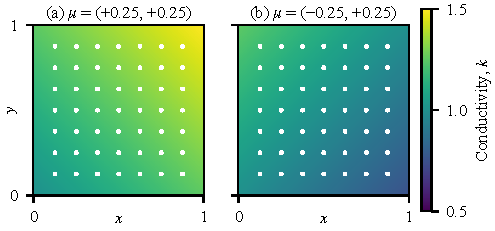
\includegraphics[width=\columnwidth]{conductivity-family.pdf}
\caption{Candidate conductivity $k=1+\mu_1x+\mu_2y$ at two corners of the parameter box. The white dots sketch a shared output grid; their spacing is for illustration only.}
\label{fig:k}
\end{figure}

Because $k$ varies in space, the expanded operator has first-order terms:
\begin{equation}
-\nabla\cdot(k\nabla u)=-\bigl[k\,(u_{xx}+u_{yy})+k_xu_x+k_yu_y\bigr].
\label{eq:expanded}
\end{equation}
For the candidate, $k_x=\mu_1$ and $k_y=\mu_2$. Dropping these terms would solve a different equation.

Geometry, source, and boundary values do not depend on $\boldsymbol{\mu}$. This makes the workload one family, not a set of unrelated problems. Changing the geometry, varying the boundary conditions, or adding parameters is outside the study.

\subsection{Parameter Sets}
The parameter box is split into three sets. The training set is used to train the PINN. A small validation set is used to watch training. A sealed held-out set is used only at the accuracy gate. The held-out set is drawn with its own seed and includes the corners of $\Theta$. The three sets must not overlap, and the held-out set is never used for training or tuning.

\subsection{What Counts as One Query}
A query gives one unseen parameter pair $\boldsymbol{\mu}^\ast$. The answer is $u$ at the $M$ points of a fixed output grid $G$, shared by both methods. Producing the whole field is one query, not $M$ queries.

The query cost covers all the work needed for that answer. For the classical solver, this is forming the matrix, solving, and mapping the solution to $G$. For the PINN, it is filling $\boldsymbol{\mu}^\ast$ into the prepared inputs and running one batched forward pass over $G$. Moving the data to and from the device is included. Neither method is charged twice for an identical query. Query blocks contain new parameter settings only, so caching gives no advantage to either side.

\subsection{Accuracy Gate and Reference}
On the grid $G$, the error of an answer $\hat u$ is
\begin{equation}
\varepsilon(\boldsymbol{\mu})=\frac{\lVert\hat u(\cdot;\boldsymbol{\mu})-u_{\mathrm{ref}}(\cdot;\boldsymbol{\mu})\rVert_2}{\lVert u_{\mathrm{ref}}(\cdot;\boldsymbol{\mu})\rVert_2}.
\label{eq:err}
\end{equation}
The primary targets are $10^{-2}$ and $10^{-3}$. The target $10^{-4}$ is optional and is attempted only within the training budget.

The reference $u_{\mathrm{ref}}$ comes from finer grids, with a Richardson check of its error. The classical solver is therefore not its own ground truth. A reference-error allowance is fixed before the gate.

A method passes a target only on the held-out set. The team still has to choose between two rules. Under the worst-case rule, every held-out parameter must meet the target. Under the quantile rule, a stated share must. The worst-case rule is stricter, and it fits the fact that the hardest corner of the box may fail first. Whichever rule is chosen applies to both methods.

Energy trials for a target begin only when both methods pass it. A method that misses is recorded as a result and kept out of the cost comparison. An inaccurate fast answer and an accurate slow answer do not solve the same task~\cite{mcgreivy2024}. A low training loss is not a pass. Only the error~\eqref{eq:err} decides.

% ===========================================================================
\section{Break-Even Model}\label{sec:model}

This section turns the question into numbers that can be measured.

\subsection{Cumulative Cost Lines}
Fix one workload, one machine, and one target. After $N$ queries, the total energy of each method is
\begin{equation}
E_P(N)=S_P+N e_P,\qquad E_C(N)=S_C+N e_C .
\label{eq:cost}
\end{equation}
Here $S$ is the one-time setup energy, and $e$ is the mean energy per query. The subscripts $P$ and $C$ mark the PINN and the classical solver. The two lines meet at
\begin{equation}
\Nstar_E=\frac{S_P-S_C}{e_C-e_P}.
\label{eq:nstar}
\end{equation}
In the usual case, the PINN has the larger setup cost, $S_P>S_C$. It can then catch up only if each of its queries is cheaper, $e_P<e_C$.

The runtime model has the same form. Let $T$ be the upfront time and $t$ the mean time per query. The runtime crossover is
\begin{equation}
\Nstar_T=\frac{T_P-T_C}{t_C-t_P}.
\label{eq:ntime}
\end{equation}
A faster method need not use less energy. So $\Nstar_E$ and $\Nstar_T$ may differ, and both are reported.

The structure follows the amortization law of Huang et~al.~\cite{huang2026review}. Our model differs in three ways. Both methods carry a setup term. The inputs are measured, not modeled. The PINN is trained from the PDE alone, so no classical solves are needed as training data.

\subsection{Setup Cost and Failed Runs}
The PINN's setup must include the cost of failure. Let $\bar E_{\mathrm{train}}$ be the mean energy of one training attempt under the frozen budget. Let $q$ be the share of attempts that pass the gate. Suppose the policy is to retrain until an attempt passes. Then the expected number of attempts is $1/q$, and
\begin{equation}
S_P=S_{\mathrm{prep}}+S_{\mathrm{val}}+\bar E_{\mathrm{train}}/q .
\label{eq:retry}
\end{equation}
The term $S_{\mathrm{prep}}$ covers model setup and loading. The term $S_{\mathrm{val}}$ is explained in the next subsection.

The policy also caps the number of attempts. If no attempt passes within the cap, the PINN fails that target. This is a valid result, not a missing one. When several seeds are trained, the deployed model is the one with the lowest validation error. All seeds trained under the policy are charged, not only the winner. Hyperparameter tuning energy is reported as a separate variant, $S_P^{+}=S_P+E_{\mathrm{tune}}$. A reader can then see how much the answer depends on tuning.

\subsection{Cost of Checking Accuracy}
Both methods need reference solutions to show that they are accurate. The PINN needs them to watch validation error and to apply its stop rule. These reference solves are classical solves. The classical solver needs a grid study to find the coarsest grid that passes each target.

We charge these costs in the same way on both sides. $S_{\mathrm{val}}$ holds the PINN's validation reference solves and its training monitoring. $S_C$ holds the classical grid study. We report each crossover twice: with these accuracy-checking terms and without them. This shows how much the answer depends on them. Table~\ref{tab:terms} lists every cost term.

\begin{table}[t]
\caption{What each cost term includes}
\label{tab:terms}
\centering
\footnotesize
\setlength{\tabcolsep}{3pt}
\begin{tabular}{@{}lp{6.5cm}@{}}
\toprule
Term & Contents \\
\midrule
$S_C$ & Grid, sparsity pattern, $A_0,A_1,A_2$, output map, grid study \\
$e_C$ & Form $A(\boldsymbol{\mu}^\ast)$, solve, map the result to $G$ \\
$S_P$ & Model setup, validation solves, monitoring, mean training energy divided by pass rate $q$ \\
$S_P^{+}$ & $S_P$ plus hyperparameter tuning energy \\
$e_P$ & Fill $\boldsymbol{\mu}^\ast$, one forward pass on $G$, return the output \\
Ledger & Every run: pilot, tuning, validation, failures, repeats \\
\bottomrule
\end{tabular}
\end{table}

\subsection{Four Outcome Classes}
A single number $\Nstar$ can mislead. It can be negative, very large, or too uncertain to trust. So each result is placed in one of four classes. Let $\Delta S=S_P-S_C$ and $\Delta e=e_C-e_P$. Let $N_{\max}$ be the largest query count reached in the trials. The intervals come from Section~\ref{sec:measure}.

First, look at the slopes. If the 95\% interval of $\Delta e$ contains zero, the per-query costs cannot be told apart. The result is then an uncertain crossing. Otherwise, let $I$ be the 95\% interval of $\Nstar=\Delta S/\Delta e$. Fig.~\ref{fig:outcomes} sketches the four classes:
\begin{enumerate}
\item \emph{Crossing in measured range}: $I\subset(0,N_{\max}]$. The crossing lies inside the measured data.
\item \emph{One method cheaper throughout}: $I$ lies at or below zero. Then $\Delta S$ and $\Delta e$ have opposite signs. One method has both the lower setup and the lower per-query cost, and the lines never cross for $N\ge0$.
\item \emph{Uncertain crossing}: $I$ straddles zero or $N_{\max}$, or the slopes cannot be told apart. No reliable crossover can be claimed.
\item \emph{Extrapolated crossing}: $I$ lies above $N_{\max}$. The crossing exists only if the lines stay straight beyond the data. It is reported as an extrapolation.
\end{enumerate}
For classes 1 and 4, we also state which method is cheaper after the crossing. If both $\Delta S$ and $\Delta e$ are negative, for example, the classical solver becomes cheaper after $\Nstar$. The same rule is applied to energy and to runtime, and their classes may differ.

\begin{figure}[t]
\centering
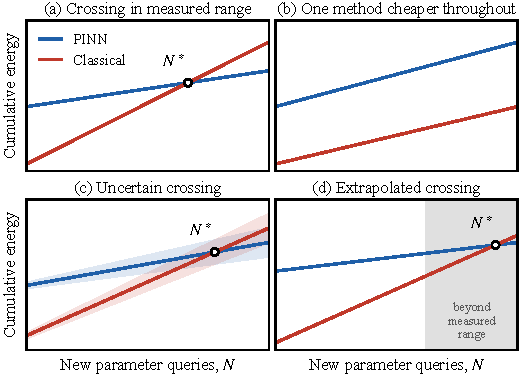
\includegraphics[width=\columnwidth]{breakeven-outcomes.pdf}
\caption{The four outcome classes. The curves are sketches, not data. Bands in (c) show uncertainty. The gray area in (d) lies beyond the largest measured query count.}
\label{fig:outcomes}
\end{figure}

\subsection{Uncertainty of the Crossover}
The crossover is a ratio, and ratios with small denominators are unstable. A first-order (delta method) estimate shows this:
\begin{equation}
\operatorname{Var}(\Nstar)\approx\frac{\operatorname{Var}(\Delta S)}{\Delta e^{2}}+\frac{\Delta S^{2}\,\operatorname{Var}(\Delta e)}{\Delta e^{4}} .
\label{eq:delta}
\end{equation}
When the gap in per-query cost $\Delta e$ is small, the second term grows with its fourth power in the denominator. The interval of $\Nstar$ then becomes wide. This is why the rule checks $\Delta e$ first. The main interval comes from a bootstrap, described in Section~\ref{sec:measure}. Equation~\eqref{eq:delta} serves as a cross-check.

\subsection{Research Questions}
The study asks four questions. None of them has an assumed answer.
\begin{itemize}
\item[Q1.] Does an energy crossover exist within a practical query count?
\item[Q2.] Do the energy and runtime crossovers fall at the same $N$?
\item[Q3.] How does $\Nstar$ move when the target tightens from $10^{-2}$ to $10^{-3}$?
\item[Q4.] How wide is the spread of $\Nstar$ across training seeds, and does a crossover claim survive it?
\end{itemize}
For Q3, a linear-model analysis suggests that tighter tolerances raise training cost~\cite{deryck2024}. A preprint finds classical solvers gaining ground as the target tightens~\cite{huangstuart2026}. We treat both as priors to test, not as results.

% ===========================================================================
\section{Classical Solver Design}\label{sec:classical}

The classical side must be efficient. Otherwise any crossover is suspect~\cite{mcgreivy2024}. This section explains how the design keeps the solver strong.

\subsection{Discretization}
The solver uses five-point finite differences on a uniform $n\times n$ interior grid with spacing $h$. The conductivity is taken at the cell faces. At an interior point $(i,j)$, the discrete equation is
\begin{multline}
\frac{1}{h^{2}}\Bigl[k_{i+\frac12,j}(u_{i,j}-u_{i+1,j})+k_{i-\frac12,j}(u_{i,j}-u_{i-1,j})\\
+k_{i,j+\frac12}(u_{i,j}-u_{i,j+1})+k_{i,j-\frac12}(u_{i,j}-u_{i,j-1})\Bigr]=f_{i,j}.
\label{eq:stencil}
\end{multline}
This keeps the flux balance correct for a varying $k$. The resulting matrix is sparse, symmetric, and positive definite. How $k$ is evaluated at the faces is fixed in the pilot, along with a convergence check.

\subsection{Affine Split and Reuse}
For the candidate~\eqref{eq:k}, $k$ is linear in the parameters. If $k$ is read at the face midpoints, each face value is linear in $\boldsymbol{\mu}$ too. The matrix then splits into three fixed parts:
\begin{equation}
A(\boldsymbol{\mu})=A_0+\mu_1A_1+\mu_2A_2 .
\label{eq:affine}
\end{equation}
$A_0$, $A_1$, and $A_2$ are assembled once, from the conductivities $1$, $x$, and $y$. A harmonic average at the faces would break this split, which is one reason the face rule is fixed early.

The split is the classical solver's main form of reuse. Each query forms $A(\boldsymbol{\mu}^\ast)$ with two scaled sparse additions. The grid, the sparsity pattern, and the output map are also reused. A factorization is not reused across queries, because the matrix changes with $\boldsymbol{\mu}$. A preconditioner may be reused only if the pilot shows that every solve still meets its tolerance.

\subsection{Solver and Grid Choice}
The pilot compares a sparse direct solve with preconditioned CG on the pilot grids. It keeps the faster one, and the choice is then frozen. For each target, the solver uses the coarsest grid in a refinement sequence that passes the gate. A finer grid would waste work and make the baseline look weaker than it is. The grid study that finds this grid is charged to $S_C$.

\subsection{Per-Query Work}
Each query forms the matrix, solves, and maps the result to $G$. These three steps are timed and measured separately. CG iteration counts may change with $\boldsymbol{\mu}$, so the cost per query may not be constant~\cite{zhang2026}. We record the cost of every held-out query. The linear-model check in Section~\ref{sec:measure} then tests whether a single slope $e_C$ is a fair summary. The classical solver uses 64-bit floats, and the precision of both methods is recorded.

% ===========================================================================
\section{Parametric PINN Design}\label{sec:pinn}

The PINN side must also be fair. A badly trained PINN would make the classical solver look better than it is. The design follows the project's training plan, which draws on the training literature. All settings below are candidates for the pilot to confirm or replace. Every tuning run is logged.

\subsection{Network and Inputs}
One fully connected network takes $(x,y,\mu_1,\mu_2)$. Its raw output is $v$. The inputs are scaled to $[-1,1]$ inside the model, with $\tilde x=2x-1$ and $\tilde\mu_i=4\mu_i$. Because the scaling is part of the model, automatic differentiation keeps the chain-rule factors. The candidate network has three or four hidden layers with tanh activation. Widths 32 and 64 are both tried. Weights start from Glorot initialization. Network size also sets the query cost, so the smallest network that passes within budget is kept~\cite{urban2025}.

\subsection{Exact Boundary Values}
Soft boundary penalties add a second loss term, which can compete with the residual~\cite{wang2021gradient,wang2022ntk}. We avoid that term. The zero boundary value is built into the output~\cite{sukumar2022,sun2020}:
\begin{equation}
\hat u(x,y;\boldsymbol{\mu})=x(1-x)\,y(1-y)\,v(x,y,\mu_1,\mu_2;\mathbf{w}).
\label{eq:hard}
\end{equation}
The multiplier is zero on all four edges. So $\hat u$ meets the boundary condition exactly, for any weights $\mathbf{w}$. Derivatives are taken through the whole expression, including the multiplier.

\subsection{Loss}
Training minimizes the mean squared residual at $N_r$ points sampled from $\Omega\times\Theta$:
\begin{equation}
\mathcal L(\mathbf{w})=\frac1{N_r}\sum_{i=1}^{N_r}\Bigl(k\,(\hat u_{xx}+\hat u_{yy})+\mu_1\hat u_x+\mu_2\hat u_y+f\Bigr)^2_{i}.
\label{eq:loss}
\end{equation}
The conductivity and its gradient are known in closed form. Automatic differentiation is used only for $\hat u$. No solution data is used, so training needs no classical solves. A unit test with a known solution checks that~\eqref{eq:loss} matches the divergence form.

\subsection{Two-Phase Training}
Training runs in two phases, as in several of the studies above~\cite{rathore2024,grossmann2024,markidis2021}. Adam runs first, with a learning rate of $10^{-3}$ and exponential decay. Its points are resampled at each step~\cite{wu2023}. L-BFGS then runs on a large fixed set of Sobol points, with a strong Wolfe line search. Its stop tolerances are set above the rounding level of the chosen precision. Table~\ref{tab:settings} lists the candidate settings and where they come from.

\begin{table}[t]
\caption{Candidate PINN settings for the pilot}
\label{tab:settings}
\centering
\footnotesize
\setlength{\tabcolsep}{3pt}
\begin{tabular}{@{}lp{5.6cm}@{}}
\toprule
Setting & Candidate \\
\midrule
Network & 3 or 4 tanh layers, width 32 or 64, Glorot init~\cite{urban2025,sun2020} \\
Boundary & Exact, by output multiplier~\cite{sukumar2022} \\
Precision & 64-bit unless the pilot rules it out~\cite{xu2025} \\
Adam phase & Learning rate $10^{-3}$ with decay; points resampled each step~\cite{hao2024,wu2023} \\
L-BFGS phase & Fixed Sobol set; strong Wolfe; history 50 to 100~\cite{rathore2024} \\
Loss weights & None needed with exact boundary values~\cite{wang2021gradient} \\
Seeds & At least 3 per frozen setting \\
\bottomrule
\end{tabular}
\end{table}

\subsection{Precision}
Precision affects both accuracy and cost. In 32-bit floats, PyTorch L-BFGS can stop on rounding noise and look converged when it is not~\cite{xu2025}. The candidate is therefore 64-bit floats for training and evaluation. The cost of 64-bit arithmetic depends strongly on the hardware. So the pilot measures the time and energy per step in both precisions before the choice is frozen. If 64-bit is too costly and 32-bit passes the targets, 32-bit is used. The choice is recorded for every run.

\subsection{Stopping, Selection, and Retry}
These rules change $S_P$ directly, so they are fixed before the main runs. No run is stopped by judgment. Two stop rules are under consideration. A fixed budget per target is simple. A rule that stops when the validation error meets the target is cheaper. However, it needs validation reference solves, and its result depends on how often it checks. If that rule is used, its check interval is frozen and the validation solves are charged to $S_{\mathrm{val}}$. An L-BFGS stop is not a pass. Each run records its stop reason, final gradient norm, and iteration count~\cite{rathore2024}.

At least three seeds are trained. Three seeds give a weak estimate of the pass rate, so failure counts are reported, not rates. The deployed model is the seed with the lowest validation error. All seeds trained under the policy are charged.

\subsection{Run Labels}
Each training run ends with one label, listed in Table~\ref{tab:labels}. Labels keep failures countable. A short note may add the likely cause, such as a network that is too small or an optimizer that stalled.

\begin{table}[t]
\caption{Labels for training runs}
\label{tab:labels}
\centering
\footnotesize
\setlength{\tabcolsep}{3pt}
\begin{tabular}{@{}lp{5.4cm}@{}}
\toprule
Label & Meaning \\
\midrule
passed & Meets the target under the gate rule \\
missed target & Used its budget; error above target \\
missed some & Mean error passes, some parameters fail \\
stalled & L-BFGS stopped with a large gradient norm \\
diverged & Loss or weights became NaN or infinite \\
overfit points & Low loss; error rising on fresh points \\
stopped & Stopped by a person or budget guard \\
\bottomrule
\end{tabular}
\end{table}

\subsection{Query Path}
A query needs no derivatives. The grid $G$ is fixed, so the coordinate part of the input is built once at setup. One query fills $\boldsymbol{\mu}^\ast$ into that input, runs one forward pass without gradient tracking, waits for the device to finish, and returns $\hat u$ on $G$. Loading the model is a setup cost. Everything after that is query cost.

% ===========================================================================
\section{Measurement Protocol}\label{sec:measure}

This section explains how the costs in Table~\ref{tab:terms} are measured.

\subsection{Hardware Counters and Boundary}
Energy is read from hardware counters on one controlled machine. Intel RAPL, through the powercap interface, covers the CPU package and memory~\cite{henderson2020,khan2018}. The NVIDIA management interface covers the GPU board. The default boundary includes the CPU package, memory, and GPU board, and it is read for both methods. This holds even when one device is mostly idle. Each component is also reported on its own. No device reading is called whole-machine electricity.

Energy is the counter difference over a window, with wrap-around corrected. It is not inferred from one power sample. If a needed counter is missing on the chosen machine, a modeled value may be used only with the supervisor's approval. Such a value is labeled as an estimate~\cite{lacoste2019,jay2023,bouza2023}.

\subsection{GPU Sampling Limits}
The NVIDIA sensor does not sample all of the runtime on some recent GPUs~\cite{yang2024}. Short GPU windows can therefore give wrong energy. Following the practice of Yang et~al.~\cite{yang2024}, each GPU query block lasts at least 5~s. Each block runs in four trials with random gaps between them. Samples taken while power is still rising are dropped. The pilot also measures the sensor's update period on the chosen GPU.

\subsection{Trial Blocks}
Each method and target is measured in blocks of queries. A warm-up block runs first and is not counted. Then $R$ repeated blocks of $K$ queries are measured. $K$ is set so that each block's energy is well above the counter noise. Thread counts, batching, device placement, and query order are fixed and recorded. Clocks are fixed where the hardware allows~\cite{yoo2026,mlperfpower2025}. Settings alone can change energy~\cite{chung2025}, so they are reported. Idle power is recorded once per session and reported next to the results. The main numbers are gross energy inside the boundary. Any idle-subtracted view is labeled.

\subsection{Training Windows}
Training is measured as one long window per attempt, rather than as many short phases. This avoids the GPU sampling problem for short windows. Setup, each training attempt, and the query blocks are separate windows. The validation solves and monitoring run inside the training window and are counted there.

\subsection{Estimates and the Linear-Model Check}
The per-query energy $e$ is block energy divided by $K$, averaged over blocks. $S_P$ follows~\eqref{eq:retry}, with $\bar E_{\mathrm{train}}$ and $q$ taken from all seeds. A bootstrap resamples seeds and blocks. Each resample gives one value of $\Nstar$, and the 2.5th and 97.5th percentiles give its 95\% interval.

The linear model~\eqref{eq:cost} assumes a stable cost per query. Before any $\Nstar$ is quoted, we check this for both methods. We compare per-query cost across block positions, block sizes, and held-out parameters. If the cost drifts, the model is reported as unsuitable for that range, and no $\Nstar$ is quoted.

\subsection{Study Ledger and Carbon}
All electricity used by the study is logged in a separate ledger. This includes exploration, the pilot, tuning, validation, failures, and repeated measurements. It is reported apart from the deployment cost model~\eqref{eq:retry}, as Henderson et~al. advise~\cite{henderson2020}. A reader can then compare the study's own energy use with what it found. If carbon is reported, it is a labeled conversion of measured energy with a stated regional factor~\cite{dodge2022}.

% ===========================================================================
\section{Pilot Plan}\label{sec:pilot}

The pilot turns the candidates above into a frozen protocol. No pilot run has been done. This section first lists the known risks that the pilot must address. It then lists the checks and the tests that guard the code.

\subsection{Known Risks and Their Handling}
The training and measurement literature points to specific ways the comparison could go wrong. Table~\ref{tab:risks} lists them with the design's response. Most come from the project's training plan. One row is our own inference: validation solves are a hidden setup cost unless they are charged.

\begin{table}[t]
\caption{Known risks and how the design handles them}
\label{tab:risks}
\centering
\footnotesize
\setlength{\tabcolsep}{2.5pt}
\begin{tabular}{@{}p{2.9cm}p{5.2cm}@{}}
\toprule
Risk & Handling \\
\midrule
Soft boundary terms compete~\cite{wang2021gradient,wang2022ntk} & Exact boundary values by multiplier \\
L-BFGS stops on 32-bit rounding~\cite{xu2025} & 64-bit, or tolerances above rounding; precision logged \\
L-BFGS line search ends early~\cite{rathore2024} & Stop reason logged; a stop is not a pass \\
Adam alone plateaus~\cite{markidis2021,rathore2024} & Adam, then L-BFGS \\
Low loss, high error~\cite{rathore2024} & Gate on the error, never on the loss \\
Hard corners of $\Theta$ fail first~\cite{deryck2024,krishnapriyan2021} & Corners in the held-out set; worst-case rule available \\
Stopping by judgment~\cite{chuang2022} & Frozen, quantitative stop rule \\
Best run hides cost~\cite{mishra2022,mcgreivy2024} & All seeds trained under the policy are charged \\
Validation solves unseen (our inference) & Charged to $S_{\mathrm{val}}$; grid study to $S_C$ \\
Short GPU windows~\cite{yang2024} & Blocks of at least 5~s, four trials \\
Classical cost varies with $\boldsymbol{\mu}$~\cite{zhang2026} & Cost recorded for every held-out query \\
Different precision per method~\cite{chuang2022} & Precision recorded; 64-bit preferred for both \\
\bottomrule
\end{tabular}
\end{table}

\subsection{Pilot Checks}
Each check below gets its own run record and ledger entry:
\begin{enumerate}
\item confirm counter access on the chosen machine, and record an idle and a load check;
\item measure time and energy per training step in 32-bit and 64-bit floats, on CPU and, if present, on GPU;
\item on the 1D heat problem, compare exact and soft boundary handling, and Adam alone with Adam then L-BFGS;
\item try two network sizes, to bracket accuracy and query cost;
\item try two batch sizes and two L-BFGS point counts;
\item measure the GPU sensor update period and the shortest block that gives stable energy;
\item check that L-BFGS stop reasons are recorded and that a NaN stops the run;
\item compare a sparse direct solve with preconditioned CG for the classical side.
\end{enumerate}
After these checks, one recipe per target is frozen and tagged in version control. Any later change is recorded with its reason. No change may be made to favor either method.

\subsection{Code and Tests}
Both methods share one evaluation function for the error~\eqref{eq:err} on $G$. This keeps the accuracy check identical on both sides. All run settings live in configuration files, and every run writes a record. Fast tests on the CPU guard the parts most likely to go wrong:
\begin{itemize}
\item the residual is near zero for a known solution, in both the expanded and the divergence form, with derivatives taken through the boundary multiplier;
\item $\hat u$ is exactly zero on boundary points;
\item the training, validation, and held-out sets do not overlap, and the held-out set contains the corners of $\Theta$;
\item two runs with the same seed and settings give the same loss history;
\item a NaN in the loss stops the run and marks it as failed;
\item the evaluation function gives the same result for the same inputs from either method.
\end{itemize}
These tests check the code, not the research result. They cannot show that a solver is accurate on the real problem. Only the gate does that.

% ===========================================================================
\section{Reporting Plan}\label{sec:report}

No measurements exist yet. This section shows the form the results will take. For each attempted target, Table~\ref{tab:results} will report the gate outcome, the setup and per-query costs, and the two crossovers with their classes. Each value will carry its 95\% interval. A method that misses the gate is marked, and its target gets no crossover.

Crossover plots will follow the layout of Fig.~\ref{fig:outcomes}, with measured axes and uncertainty bands. Each crossover will be shown with and without the accuracy-checking terms. The study ledger will be reported as its own table.

\begin{table}[t]
\caption{Reporting format for each target (empty until the trials)}
\label{tab:results}
\centering
\footnotesize
\setlength{\tabcolsep}{2.6pt}
\begin{tabular}{@{}llccccc@{}}
\toprule
Target & Method & Gate & $S$ (kJ) & $e$ (J) & $T$ (s) & $t$ (ms) \\
\midrule
$10^{-2}$ & PINN      & -- & -- & -- & -- & -- \\
          & Classical & -- & -- & -- & -- & -- \\
          & \multicolumn{6}{l}{Crossover: $\Nstar_E$ --, $\Nstar_T$ --; class --} \\
\midrule
$10^{-3}$ & PINN      & -- & -- & -- & -- & -- \\
          & Classical & -- & -- & -- & -- & -- \\
          & \multicolumn{6}{l}{Crossover: $\Nstar_E$ --, $\Nstar_T$ --; class --} \\
\bottomrule
\end{tabular}
\end{table}

% ===========================================================================
\section{Threats to Validity}\label{sec:threats}

\subsection{Weak Baseline}
An under-tuned classical solver can create a crossover that does not exist~\cite{mcgreivy2024}. The affine reuse, the pilot's solver choice, and the coarsest passing grid are meant to prevent this. The reuse rules are reviewed before the trials.

\subsection{Weak PINN}
A badly trained PINN can hide a crossover that does exist. The two-phase training, the precision check, and the exact boundary values are meant to prevent this. Newer optimizers~\cite{wang2025soap} or metalearning~\cite{penwarden2023} might lower the training cost further. We do not test them, so our result says nothing about them.

\subsection{Unequal Coverage}
A GPU reading and a CPU reading are not the same system total. Reading one boundary for both methods avoids this. An idle GPU then adds energy to the classical runs. For a deployment that has no GPU, the per-component view is the better guide.

\subsection{Training Variance}
Three seeds give a weak estimate of the pass rate $q$. A low $q$ raises $S_P$ and widens its interval. That can move a result into the uncertain class. We will report that outcome rather than select a lucky seed.

\subsection{Linear Model}
The cost lines assume a stable cost per query. If either method's cost drifts with $N$ or with $\boldsymbol{\mu}$, the lines do not hold. The linear-model check reports this instead of quoting $\Nstar$.

\subsection{Scope}
The results will hold only for the tested machine, PDE family, parameter box, and targets. Reduced basis methods~\cite{hesthaven2016} and multigrid solvers are strong options for many queries and for elliptic problems. We do not test them. Several of our main sources are preprints~\cite{huang2026review,huangstuart2026,zhang2026,kapoor2025}. They will be checked for published versions before the final report.

% ===========================================================================
\section{Open Decisions}\label{sec:open}

The design leaves some choices to the team. They must be made before the main runs:
\begin{itemize}
\item the gate rule: worst case or a stated quantile;
\item whether validation solves and the grid study are charged to setup, as proposed;
\item the stop rule: fixed budget or target-based;
\item the device and precision for PINN training and queries;
\item the maximum number of training attempts;
\item the machine, the counters, and the compute budget.
\end{itemize}
If the four-input network fails the gate, a different way of feeding the parameters could be tried. That would be a design change. It would need the owner's approval, and its cost would be logged.

% ===========================================================================
\section{Conclusion}\label{sec:conclusion}

A parametric PINN pays for training up front and hopes to win it back through cheap queries. This paper set out how to measure whether, and when, that happens against a finite-difference solver at the same accuracy. The design charges failed runs and the cost of checking accuracy. It reads both methods inside one energy boundary. It sorts each result into one of four outcomes, each with an interval, and it treats a missing crossover as a valid answer. The next step is the pilot. It will check the energy counters, test both methods on the 1D heat problem, and freeze the protocol.

\section*{Acknowledgment}
An AI assistant helped draft and edit this paper from the project's research notes. The authors are responsible for its content.

\bibliographystyle{IEEEtran}
\bibliography{../shared/references}

\end{document}
